\documentclass[a4paper,12pt,italian]{article}

\usepackage[T1]{fontenc} 
\usepackage[utf8]{inputenc}

\usepackage{graphicx} % Required for the inclusion of images
\graphicspath{ {Immagini/} }
\usepackage{float}
\usepackage{eurosym}

\usepackage{tikz}
\usetikzlibrary{positioning}
\definecolor{burntorange}{cmyk}{0,0.51,1,0}
\definecolor{processblue}{cmyk}{0.96,0,0,0}

\title{Progetto di Robotica \\ \large Progettazione e Sviluppo di RoboHenree} % Title


\author{Riccardo Musmeci, Carlo Nuccio, Danilo Pipitone} % Author name

\date{\today} % Date for the report


\begin{document}

\maketitle % Insert the title, author and date

\tableofcontents

\pagebreak

\section{Prefazione}
Da diversi decenni la \textit{Robotica} ha suscitato l'interessa di molti studiosi e ricercatori, spinti dall'interdisciplinarità della stessa verso settori come l'Informatica, l'Elettronica e la Meccanica. 

Oggigiorno si sente spesso parlare di IoT, Internet of Things, ossia quell’insieme di fattori hardware e software low cost, che consentono lo sviluppo di smart services a disposizione delle società ma anche della singola persona. 

Piattaforme come \textit{Arduino} e \textit{Raspberry} sono due delle più utilizzate nel campo della IoT, le quali si prestano molto bene allo sviluppo di Robot Intelligenti e non solo.

Grazie all’avvento di tali tecnologie si è data una spinta radicale verso una nuova era in cui tutti, con una conoscenza minimale, sono in grado di sviluppare idee di questo tipo in ambito industriale, domotico o semplicemente fai da te.

In questa relazione discuteremo quelle che sono state le scelte progettuali, sia hardware che software, per la realizzazione di un robot mobile, \textbf{RoboHenree}, il cui compito è quello di competere per la RoboCup organizzata dal dipartimento di Robotica dell’Università degli Studi di Palermo, per il corso di Robotica tenuto dal Prof. \textbf{Antonio Chella}.

Si ringrazia tutto lo staff del \textbf{RoboticsLab} della Scuola Politecnica, che ci ha messo a disposizione il laboratorio per provare il robot sul campo della competizione. 

Un ringraziamento particolare va al prof. Antonio Chella per averci esposto tutti gli aspetti teorici relativi alla costruzione e implementazione del nostro robot.
Inoltre, si ringrazia l’Ing. \textbf{Salvatore Tramonte} per tutti i preziosi consigli ed insegnamenti che ci ha dato al fine dello sviluppo del robot.

\section{Introduzione}
La robotica ha come scopo principale quello di creare delle macchine in grado di sostituire l’essere umano nello svolgimento di un determinato compito.
Non si limita però solo a questo, infatti altro campo di applicazione della robotica è la \textbf{Human Computer Interaction} (HCI), secondo il quale un robot è in grado di facilitare la vita dell’uomo nella sua vita di tutti i giorni.
Questo primo capitolo ha lo scopo di dare una panoramica sulle varie tipologie di robot che vengono utilizzati per le più recenti applicazioni.

\subsection{La Robotica}
Il termina "\textit{Robotica}" venne introdotto per la prima volta negli anni '40 da \textbf{Asimov} per indicare la scienza relativa allo studio dei robot basata sulle seguenti tre leggi:
\begin{itemize}
	\item Un robot non può fare del male ad un essere umano e né consentire che un umano si trovi in pericolo mentre il robot è in stato inoperoso.
	\item Un robot deve obbedire agli ordini impartiti dagli esseri umani, a meno che questi non rientrino in conflitto con la prima legge. 
	\item Un robot deve proteggere la sua esistenza a meno che non sono in conflitto con la prima e la seconda legge. 
\end{itemize}

Oggi la robotica viene definita come la scienza che studia l’interconnessione tra \textbf{percezione} e \textbf{azione}.

Un generico sistema robotico è composto da uno schema di questo tipo:
 
\begin{figure}[H]
\begin{center}
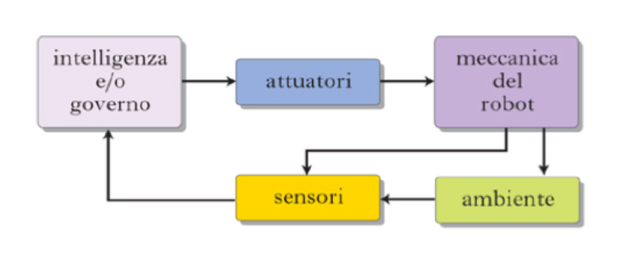
\includegraphics[width=0.65\textwidth]{robotica}
\caption{Generico sistema robotico}
\end{center}
\end{figure}

Descriviamo brevemente di cosa si occupa ciascun blocco:
\begin{itemize}
	\item \textbf{Sistema meccanico}: costituito da organi di locomozione, i quali consentono all’agente il movimento e la manipolazione al fine di interagire sugli oggetti dell’ambiente circostante. Alcuni elementi di questo sistema sono ad esempio ruote, cingoli o arti meccanici.
	\item \textbf{Attuatori}: rappresentano la capacità del robot di agire sia per muoversi che per manipolare oggetti; legati ai concetti di servomotori ed organi di trasmissione.
	\item \textbf{Sensori}: implementano la capacità percettiva dell’agente, tramite i quali il robot è in grado di acquisire informazioni sullo stato interno del robot o su quello esterno. La realizzazione di un sistema siffatto è legata all’acquisizione dei segnali, alla loro elaborazione ed all’estrazione delle informazioni ad essa associate.
	\item \textbf{Governo}: rappresenta la capacità di connettere in maniera intelligente azione e percezione. Tale sistema è in grado di guidare l’esecuzione dell’azione nel rispetto degli obiettivi imposta da una pianificazione del compito e dai vincoli imposti dal robot e dall’ambiente.
\end{itemize}

\subsection{Tipi di schede}
Abbiamo già introdotto le schede Arduino e Raspberry, è importante adesso capire analogie e differenze. 

Arduino è un microcontrollore e come tale, possiede caratteristiche computazionali inferiori rispetto a qualsiasi altro dispositivo capace di emulare un computer. Schede come Arduino sono in grado di leggere un determinato input e trasformarlo in un output sotto forma di un’azione, come l’attivazione di un motore, l’accensione di un LED o qualsiasi altro comando inviato ad un attuatore. Inoltre he delle GPIO sia analogiche che digitali, a differenza del Raspberry per il quale sono solo digitali. 

Una valida alternativa è il Raspberry, il quale non è un microcontrollore ma un vero e proprio computer in miniatura. A confermare quanto detto sono le componenti che troviamo montate sulla scheda come la CPU, le porte USB e HDMI ecc. Inoltre, una cosa fondamentale che lo distingue totalmente dall’Arduino è che su questa scheda si deve montare un sistema operativo. Quello di default è il Raspbian OS, una distribuzione Linux derivata da Debian. Questo fa sì che, mentre l’Arduino viene utilizzato come un microcontrollore a cui ad un input corrisponde un’azione in output, nel Raspberry si possono fare girare tutti i software che vogliamo nel linguaggio che desideriamo. Quindi, sulla board stessa possiamo fare qualsiasi tipo di elaborazione dei segnali in input e trasformarli in output senza dover passare ad un server di elaborazione come avviene per Arduino.

\begin{figure}[H]
\centering
\begin{minipage}{.5\textwidth}
  \centering
  
\includegraphics[scale=0.5]{arduino_symbol}
  \caption{Arduino}
  \label{fig:arduino_symbol}
\end{minipage}%
\begin{minipage}{.5\textwidth}
  \centering
  
\includegraphics[scale=0.5]{raspberry}
  \caption{Raspberry}
  \label{fig:raspberry}
\end{minipage}
\end{figure}

\subsubsection{Confronto}
Una volta descritte le funzionalità e le caratteristiche di Arduino e Raspberry, facciamo un confronto diretto tra le due possibili alternative. Nell’ambito del nostro progetto, si possiede un budget massimo di 100 Euro, questo ci ha portato a dover scegliere una delle due. Dal punto di vista della costruzione fisica del robot, non vi è alcuna differenza, poiché per entrambe vanno scelte accuratamente le singole componenti da montare nel proprio robot. Alla fine abbiamo scelto Arduino che, essendo un semplice microcontrollore, deve soltanto eseguire dei comandi ricevuti in input e non può essere fatta alcun tipo di elaborazione a causa delle risorse limitate. Questo impone, necessariamente, un’architettura client-server, dove il secondo dovrà elaborare le informazioni per l’Arduino. Questo tipo di architettura consente una velocità di analisi dei dati provenienti dai sensori molto elevata a discapito di una comunicazione più lenta rispetto a quelle del Raspberry. Elenchiamo adesso i pro e i contro di tale scelta.	
       
I pro sono:
\begin{itemize}
	\item Costo Basso.
	\item Elevate prestazioni server side. 
	\item Possibilità di manipolare le componenti. 
	\item Facilità di interazione col mondo esterno. 
	\item Uso di librerie già implementate per le diverse componenti. 
\end{itemize}

I contro sono:
\begin{itemize}
	\item Complessità nella gestione sincronizzata delle varie risorse.
	\item Sviluppo di protocolli di comunicazione flessibili e leggeri.
	\item Difficoltà nell’esecuzione di azioni percezione-azione qualora sono coinvolte elaborazioni visuali. 
\end{itemize}

Come già detto, la nostra scelta è caduta su Arduino in quanto abbiamo preferito avere una architettura client-server, dove il client, ovvero Arduino, si occupa della parte reattiva del robot, mentre il server funge da "direttore" per il client, utilizzando le elevate prestazioni computazionali a disposizione, decidendo così le azioni che il robot deve compiere.

\section{La RoboCup}

La \textbf{RoboCup} è la competizione organizzata dal \textit{RoboticsLab} per gli studenti del corso di laurea magistrale in Ingegneria Informatica. Tale competizione rappresenta un modo per promuovere la ricerca e la sperimentazione nel campo della robotica e dell'intelligenza artificiale. 


\subsection{La competizione e le regole}

La RoboCup per l'anno accademico 2016/2017 prevede la costruzione di un robot in grado di muoversi all'interno di un mondo, in cui sono presenti degli ostacoli, posizionati casualmente, con l'obiettivo di raggiungere degli oggetti, posizionati in una determinata area del mondo, per poi riportarli in determinate aree associate, in base al colore, agli oggetti stessi.

Le fasi della competizione sono due:
\begin{itemize}
	\item \textbf{Fase BCI (Opzionale)}: in questa fase i partecipanti dovranno riconoscere la presenza di potenziali evento correlati (ERP- P300) in un tracciato cerebrale.
	\item \textbf{Fase match (Obbligatoria)}: scopo della competizione è quello di realizzare un robot autonomo in grado di identificare dei bersagli di forma e dimensione differente e di riportali nell’appropriata area goal.
\end{itemize}

La fase BCI richiede di discriminare i seguenti comandi:
\begin{figure}[H]
\begin{center}
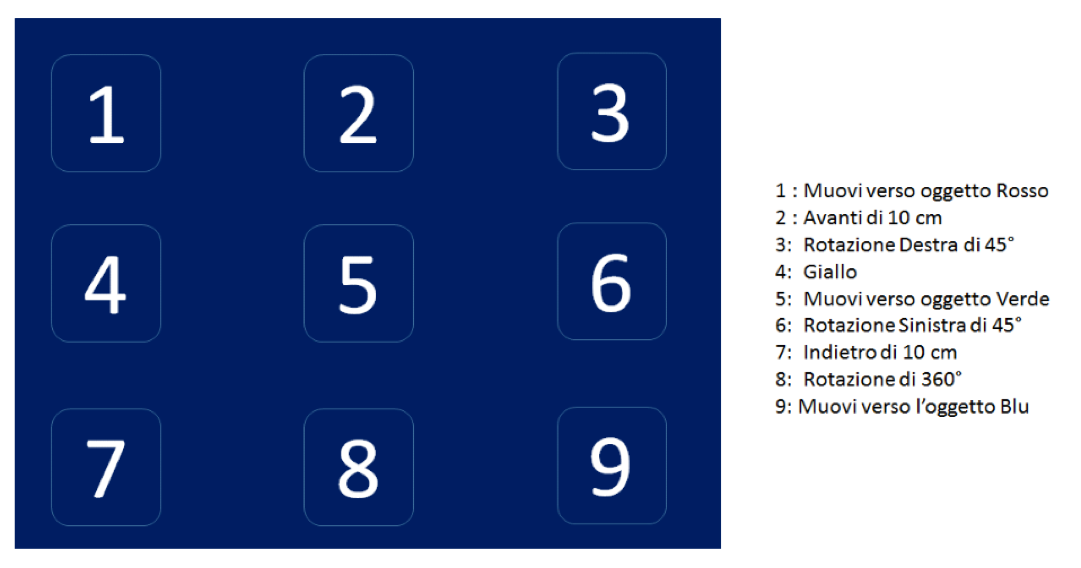
\includegraphics[scale=0.4]{BCI}
\caption{Comandi BCI}
\end{center}
\end{figure}

La mappa generale in cui il robot dovrà muoversi è la seguente.

\begin{figure}[H]
\begin{center}
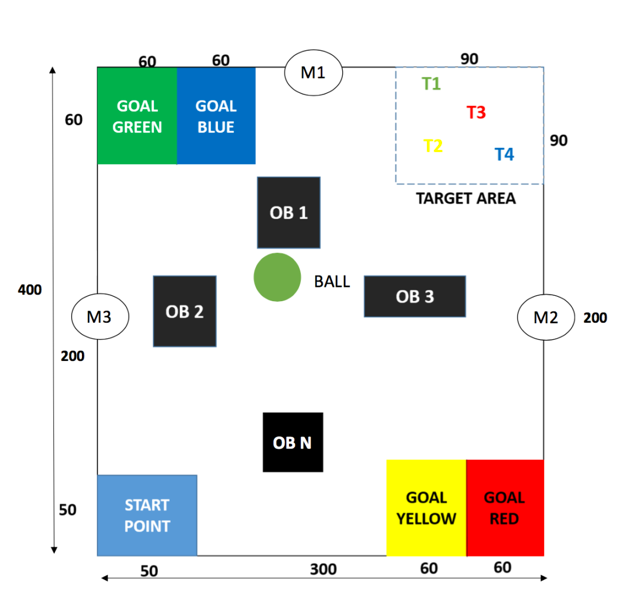
\includegraphics[scale=0.5]{mappa}
\caption{Mappa generica della RoboCup}
\label{Fig:mappa}
\end{center}
\end{figure}

Le regole generali previste dalla RoboCup sono le seguenti.
\begin{itemize}
	\item \textbf{Obiettivo}: individuare e raccogliere i target trasportandoli all'appropriata area goal.
	\item \textbf{Durata}: 
		\begin{itemize}
			\item BCI (Opzionale): 5 minuti
			\item Match: 10 minuti effettivi di gioco più un tempo bonus
		\end{itemize}
	\item \textbf{Timeout}: Il referente di Team può chiedere un timeout (max 2 volte per un tempo massimo totale di 5 minuti) al fine di modificare le impostazioni hardware e software del robot. L’hardware del robot può essere sostituito con altro hardware solo se precedentemente presentato e computato nella lista dell’hardware accettato dalla commissione.
	\item \textbf{Tempo bonus}: Il bonus è conteggiato in secondi. Si guadagnano 6 sec di bonus ogni euro risparmiato. La stima è effettuata per arrotondamento all’intero più vicino (1.7 euro = 12 secondi).
	\item \textbf{Budget}: : La spesa massima del progetto deve essere di 100\euro{}. Ogni componente hardware deve essere corredato da bolla di acquisto o dal prezzo di mercato (sito del produttore) al fine di comprovarne il valore.
	\item Il robot deve essere autonomo.
	\item Il robot deve avere una dimensione massima di 30X40X40 cm.
	\item Il campo ha dimensioni descritte in Fig. \ref{Fig:mappa} (le dimensioni sono espresse in cm).
	\item All’interno del campo sono presenti un numero variabile di ostacoli, la cui posizione non è nota indicati con OB.
	\item La distanza minima fra due ostacoli è tale da consentire il passaggio del robot.
	\item Due o più ostacoli possono essere posizionati di seguito.
	\item La collisione che porta ad uno spostamento degli ostacoli o alla loro caduta implica una penalità. L’assegnazione della penalità è valutata dai giudici.
	\item Il robot parte dallo start point rivolto verso il Nord del campo (GOAL GREEN).
	\item Sono presenti 3 landmark M1, M2 ed M3 nelle posizioni indicate.

\end{itemize}


Le due fasi di gioco presentano delle regole distinte.

Le regole per la fase BCI sono:
\begin{itemize}
	\item Il robot è posizionato nello start point
	\item Il giorno della competizione viene fornito un tracciato cerebrale di training contente P300 ERPs correlati dai label ad essi associati ed un tracciato cerebrale contenente esclusivamente gli ERPs. Il robot deve riconoscere il comando associato ed eseguire l’azione corrispondente.
	\item Il robot dovrà fermarsi ad una distanza compresa fra 1 e 5 cm dal target BCI (se l’azione richiesta è l’avvicinamento).
	\item La corretta selezione del comando e l’esecuzione della corrispondente azione assegna un numero variabile di punti (vedi sezione calcolo punteggio).
	\item La corretta selezione del comando consente la rimozione di un ostacolo a scelta dei giudici
	\item Al termine della fase BCI gli oggetti sono posti nell’area assegnata ed il robot è posizionato nuovamente nello starting point.
	\item Il tracciato cerebrale presenta le seguenti caratteristiche:
		\begin{itemize}
			\item Acquisizione a 256 Hz.
			\item Paradigma di illuminazione Riga – Colonna di un’interfaccia di dimensioni 3x3.
			\item Ciascun elemento dell’interfaccia è stato illuminato 8 volte ( 4 per riga, 4 per  colonna).
			\item Il tracciato cerebrale è fornito in formato .bin e contiene 7 canali. I canali da 1 ad 4  contengono il valore registrato dal canale corrispondente espresso in uVolt; il  canale 5 indica il trial, il canale 6 contiene gli eventi relativi al simbolo  dell’interfaccia illuminato; il canale 7 non contiene informazioni rilevanti per la  competizione.
			\item I tracciati di calibrazione vengono denominati CalibXXXX.bin dove ciascuna “X” indica il simbolo dell’interfaccia su cui si è focalizzata l’attenzione (Calib123.bin  indica che ci si è focalizzati sul simbolo 1, successivamente sul 2, successivamente sul 3).
		\end{itemize} 
\end{itemize}

Le regole per il match sono:
\begin{itemize}
	\item Il match ha inizio con il robot posizionato nello starting point.
	\item I target indicati in figura con la T sono presenti all’interno della target Area. La target Area non è marcata sul campo, ma ha dimensione e posizione fissa e tutti i target si trovano all’interno di tale area.
	\item I target T devono essere presi uno alla volta.
	\item I target T hanno forma e colori differenti.
	\item Ciascun target T deve essere portato nell’area goal il cui colore corrisponde al target. 
	\item I target T hanno un valore differente (vedi sezione punteggi) green goal T3 – red goal etc..).
	\item Se un target è portato nell’errata area goal è assegnata una penalità ma il target non è rimesso in gioco.
	\item In aggiunta ai target, è presente una palla verde (BALL) la cui posizione nel campo è casuale.
	\item La palla verde deve essere riportata in una qualunque area goal DOPO aver trasportato almeno un target all’interno della appropriata aree goal.
	\item Se la palla è accidentalmente spinta in un’area goal, prima degli altri target, la palla viene posizionata manualmente in una nuova posizione del campo e nessuna penalità è assegnata.
	\item Se il robot riporta nella corretta area goal tutti i target più la palla verde prima dello scadere del tempo, la competizione è considerata conclusa e viene computato un bonus di 3 punti per ogni secondo risparmiato rispetto al tempo limite.
\end{itemize}

I punteggi assegnati per la classifica finale sono, in base alle fasi, i seguenti.

\begin{center}
	\begin{tabular}{ |p{3cm}||p{4cm}|p{3cm}| }
 		\hline
 		\multicolumn{3}{|c|}{Fase BCI - 30 punti max} \\
 		\hline
 		Comando & Corretta Selezione & Corretta Azione \\
 		\hline
		 CMD 1 & 8 & 2\\
 		 CMD 2 & 8 & 2\\
 		 CMD 3 & 8 & 2\\
		\hline
	\end{tabular}
\end{center}

\begin{center}
	\begin{tabular}{ |p{5cm}||p{3cm}| }
 		\hline
 		\multicolumn{2}{|c|}{Fase Match} \\
 		\hline
 		Oggetto & Valore\\
 		\hline
		 Piramide Blu & 5\\
 		 Elle Gialla & 10\\
 		 Palla Verde & 20\\
 		 Pillola Blu & 15\\
 		 Parallelepipedo Rosso & 5\\
		\hline
	\end{tabular}
\end{center}

\begin{center}
	\begin{tabular}{ |p{5cm}||p{3cm}| }
 		\hline
 		\multicolumn{2}{|c|}{Penalità} \\
 		\hline
 		Tipologia & Valore\\
 		\hline
		 Ostacolo abbattuto o spostato & -3\\
 		 Oggetto portato nell'area goal non corretta & -10\\
 		 Palla portata in un'area gola prima di aver portato a destinazione un oggetto & -15\\
		\hline
	\end{tabular}
\end{center}

\section{Hardware}
Questa sezione illustra dettagliatamente le componenti hardware usate per costruire il robot.

\subsection{Arduino}
Il robot è stato costruito utilizzando Arduino e non Raspberry. Il tipo di Arduino scelto è il \textit{Mega 2560 R3}.

\begin{figure}[H]
\begin{center}
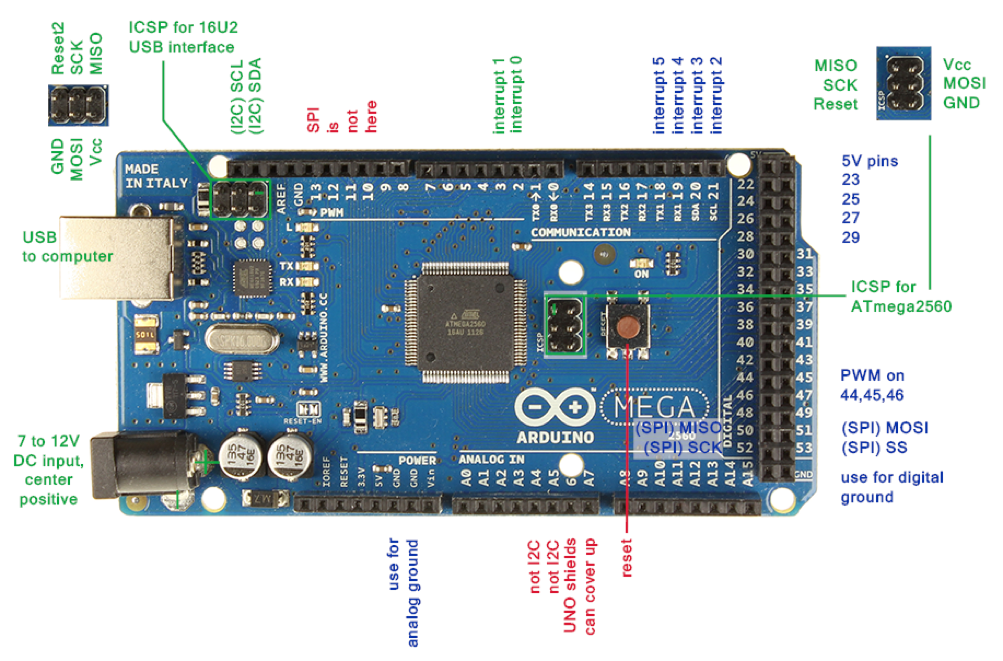
\includegraphics[scale=0.6]{arduino}
\caption{Arduino Mega 2560 R3}
\label{Fig: arduino}
\end{center}
\end{figure}

Come mostra la Figura \ref{Fig: arduino}, questo modello possiede 54 pin di input/output, 16 pin analogici e 4 porte seriali. Inoltre possiede un oscillatore a 16 MHz, una memoria di 256 KB e una porta USB. Rispetto all’Arduino Uno, che riportiamo sotto in Figura \ref{Fig: arduino_uno}, il modello scelto vanta di una maggiore potenza a discapito di una maggiore dimensione fisica.

\begin{figure}[H]
\begin{center}
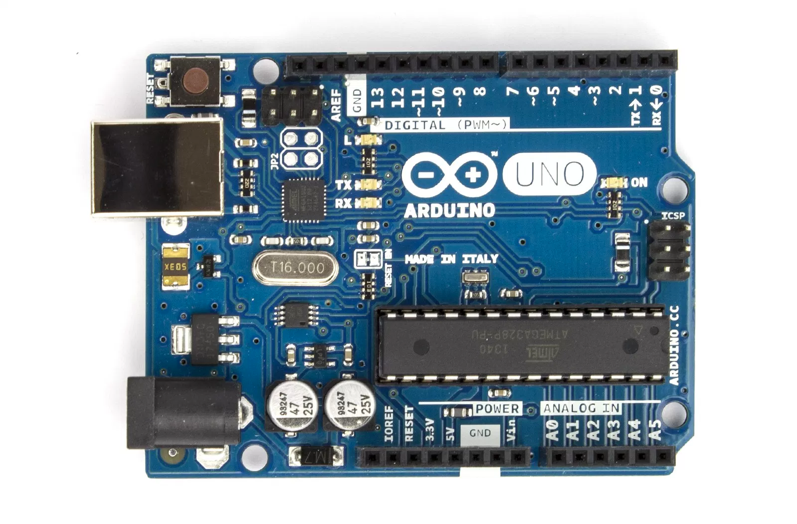
\includegraphics[scale=0.6]{arduino_uno}
\caption{Arduino Mega 2560 R3}
\label{Fig: arduino_uno}
\end{center}
\end{figure}

\subsection{Sensori}
\label{subsec: sensori}
I sensori sono dei dispositivi che permettono al robot di percepire informazioni provenienti dal mondo esterno e di interagire con esso. La percezione rende le macchine più intelligenti, le quali possono essere istruite per effettuare compiti complessi. Sono progettati per acquisire e misurare grandezze reali che hanno una qualche relazione con altre proprietà dell’ambiente che vogliamo conoscere. 

Tutti i sensori sono caratterizzati da una serie di proprietà che ne descrivono le capacità. Le più importanti sono le seguenti:

\begin{itemize}
	\item \textbf{Sensibilità}: rapporto tra la variazione dell’uscita e quella dell’ingresso.
	\item \textbf{Linearità}: misura della costanza del rapporto tra ingresso e uscita.
	\item \textbf{Intervallo di misura}: differenza tra i valori minimi e massimi misurabili. 
	\item \textbf{Tempo di risposta}: tempo necessario affinché una variazione unitaria dell’ingresso 
mostri i suoi effetti in uscita. 
	\item \textbf{Accuratezza}: differenza tra il valore vero e il valore misurato. 
	\item \textbf{Ripetibilità}: differenza tra due misurazioni successive della stessa entità. 
	\item \textbf{Risoluzione}: il più piccolo incremento osservabile all’ingresso. 
	\item \textbf{Tipo di uscita}. 
\end{itemize}

Inoltre, la funzione dei sensori di un robot può essere ripartita in due categorie principali: 
\begin{itemize}
	\item Sensori dello stato interno: riguardano la misura di variabili, che sono usate per il controllo del robot. 
	\item Sensori dello stato esterno: trattano la misura di variabili quali la distanza, la prossimità e il tatto. La percezione esterna, è utilizzata per la guida del robot e inoltre per l'identificazione degli oggetti. 
\end{itemize}

Dopo aver fatto una panoramica sull’importanza dei sensori per un robot, analizziamo in dettaglio ogni singola componente utilizzata nel nostro progetto.
\begin{itemize}
	\item \textbf{Sensori infrarossi}: sono dei sensori che	permettono di stabilire la presenza di oggetti o ostacoli nelle vicinanze del robot. Operano mediante l’emissione di una luce infrarossa e il rilevamento della sua riflessione dovuta alle superfici poste di fronte al robot. Se tutti gli oggetti dell’ambiente in cui opera il robot abbiano una struttura con colori e superfici uniformi, i sensori a infrarosso possono essere calibrati in modo da misurare le distanze dagli oggetti. La massima distanza rilevabile è solitamente compresa tra 50 e 100 cm. Il nostro robot monta 9 sensori TE174, come quello mostrato in Figura \ref{Fig: ir}. 
		\begin{figure}[H]
			\begin{center}
			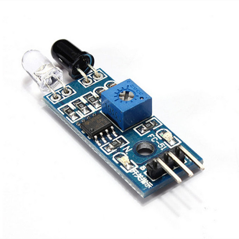
\includegraphics[scale=0.6]{ir}
			\caption{Sensore ad infrarosso}
			\label{Fig: ir}
			\end{center}
		\end{figure}
		Di questi 9 sensori, 4 sono stati posizionati nella parte frontale del robot, due nelle parti laterali, e 3 sulla barra utilizzata per catturare l'oggetto, e 1 per determinare la vicinanza con l'oggetto da prendere.
	\item \textbf{Bussola}: è un sensore che permette di misurare i campi magnetici nelle direzioni x, y, z. Può essere utilizzato in modi differenti, per esempio per misurare il campo magnetico terrestre oppure per rilevare la presenza di ostacoli nelle vicinanze. Per il nostro robot è stato scelto il modulo HMC5883L, come quello mostrato in Figura \ref{Fig: bussola} .
		\begin{figure}[H]
			\begin{center}
			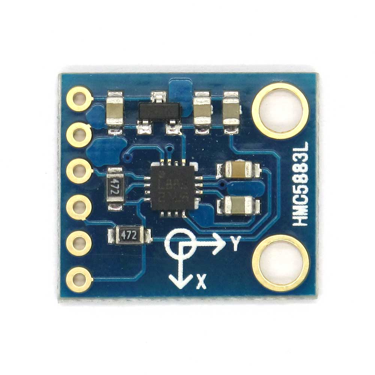
\includegraphics[scale=0.4]{bussola}
			\caption{Bussola HMC5883L}
			\label{Fig: bussola}
			\end{center}
		\end{figure}
		Esso è stato scelto per dare al robot la capacità di orientarsi all’interno dello spazio di gioco. Questo sensore permette di capire come è orientato il robot rispetto al nord terrestre, a monte però bisogna calibrare opportunamente, tenendo conto di due fattori fattori fondamentali ovvero la declinazione magnetica e gli offset che permettono una lettura più accurata dei valori a run-time. 
	\item \textbf{Camera}: la camera è uno dei sensori più importanti per qualsiasi robot perché permette di vedere “con occhi” il mondo esterno. Esistono diverse tipologie di camera, per il nostro progetto abbiamo utilizzato una Camera IP come quella mostrata in Figura \ref{Fig: camera}.
		\begin{figure}[H]
			\begin{center}
			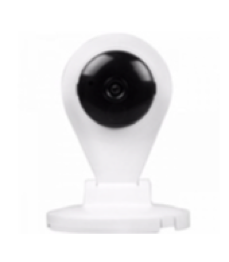
\includegraphics[scale=0.4]{camera}
			\caption{Camera IP}
			\label{Fig: camera}
			\end{center}
		\end{figure}
	\item \textbf{Modulo Wi-Fi}: è il modulo che permette ad Arduino di inviare dati ad un server tramite protocollo TCP.
		\begin{figure}[H]
			\begin{center}
			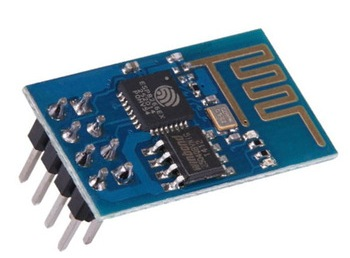
\includegraphics[scale=0.2]{wifi}
			\caption{Modulo Wi-Fi}
			\label{Fig: wifi}
			\end{center}
		\end{figure}

\end{itemize}

\subsection{Attuatori}
Un attuatore è un meccanismo che permette ad un agente, anche artificiale,  di agire nell’ambiente in cui si trova sulla base degli stimoli ricevuti. Mentre, i sensori consentono di percepire il mondo circostante, gli attuatori permettono di interagire fisicamente con esso. Di seguito un elenco degli attuatori utilizzati per il nostro progetto.

\begin{itemize}
	\item \textbf{Servo motore}: La sua caratteristica principale è che può ruotare nell’intervallo [0-180] in entrambi i versi. Inoltre, sopporta un peso al massimo di 9 grammi ed è stato utilizzato per poter abbassare la bacchetta per poter intrappolare gli oggetti.
 		\begin{figure}[H]
			\begin{center}
			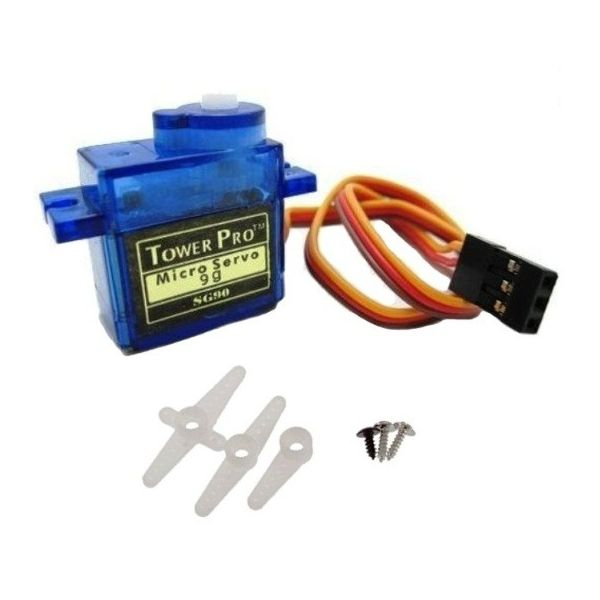
\includegraphics[scale=0.1]{servo}
			\caption{Servo SG90}
			\label{Fig: servo}
			\end{center}
		\end{figure}
	\item \textbf{Stepper Controller}: è un circuito integrato che facilita l'utilizzo dei motori DC. Questo circuito integrato è composto da due ponti ad H. Il ponte H è una particolare configurazione elettronica che permette di invertire la marcia/direzione dei motori utilizzando un segnale di comando a 5V TTL. Il modello comprato è il L298N.
		\begin{figure}[H]
			\begin{center}
			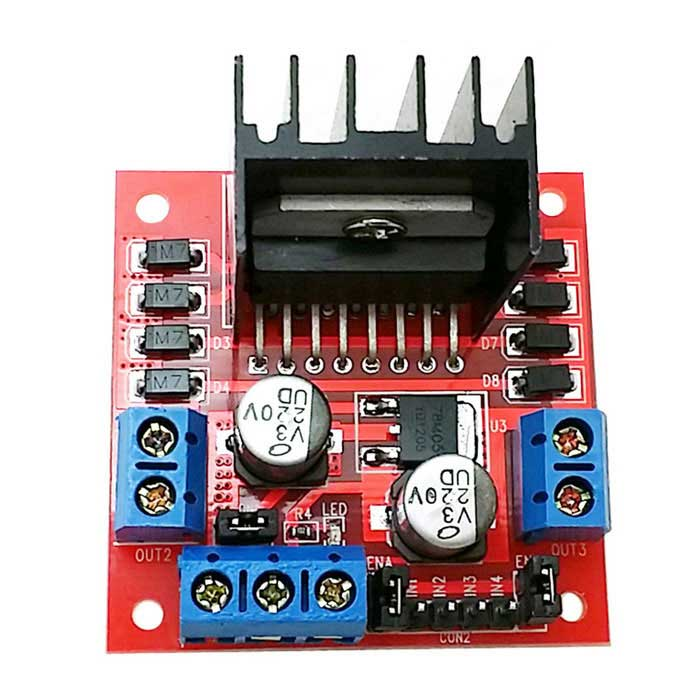
\includegraphics[scale=0.1]{l298n}
			\caption{Modulo L298N}
			\label{Fig: driver}
			\end{center}
		\end{figure}
	\item \textbf{Motori DC}: sono i motori che permettono il movimento delle ruote del robot.
\end{itemize}


\section{Software}
Questa sezione illustra tutti gli strumenti che sono stati utilizzati per la progettazione e l'implementazione del software del robot.

\subsection{Python}
Python è il linguaggio scelto per l'implementazione di alcune parti software del nostro robot.
Python è un linguaggio di programmazione ad alto livello, rilasciato per la prima volta nel 1991 dal suo creatore Guido Van Rossum. Lo sviluppo di Python è in continua crescita grazie ad una grande e dinamica comunità internazionale di sviluppatori e viene gestito dall'organizzazione no-profit Python Software Foundation. 

Tale linguaggio supporta diversi paradigmi di programmazione, come quello object-oriented (con supporto all'ereditarietà multipla), quello imperativo e quello funzionale, ed offre una tipizzazione dinamica forte. È fornito di una libreria built-in estremamente ricca, che unitamente alla gestione automatica della memoria e a robusti costrutti per la gestione delle eccezioni fa di Python uno dei linguaggi più ricchi e comodi da usare. 

Python è un linguaggio pseudo-compilato: un interprete si occupa di analizzare il codice sorgente e di eseguirlo, rendendolo quindi Python un linguaggio portabile. Una volta scritto un sorgente, esso può essere interpretato ed eseguito sulla buona parte delle piattaforme attualmente utilizzate, come Mac OS, Windows e Linux.  Semplicemente, basta la presenza della versione corretta dell'interprete. 

Infine, Python è completamente gratuito e può essere liberamente modificato e così ridistribuito, secondo le regole di una licenza pienamente open-source. Queste caratteristiche hanno fatto di Python uno dei linguaggi più utilizzati al mondo. 

\subsection{OpenCV}
OpenCV è una delle librerie più importanti utilizzata nella Computer Vision e nell’Image Processing.

Essa supporta tutti i sistemi operativi e può essere utilizzata dai principali linguaggi di programmazione, Python nel nostro caso. In particolare, tale libreria viene utilizzata per processare e riconoscere gli oggetti catturati da una camera e tramite opportuni algoritmi si è in grado di emulare la capacità visiva umana.

\section{RoboHenree}

Ecco alcune foto di RoboHenree.

\begin{figure}[H]
\begin{center}
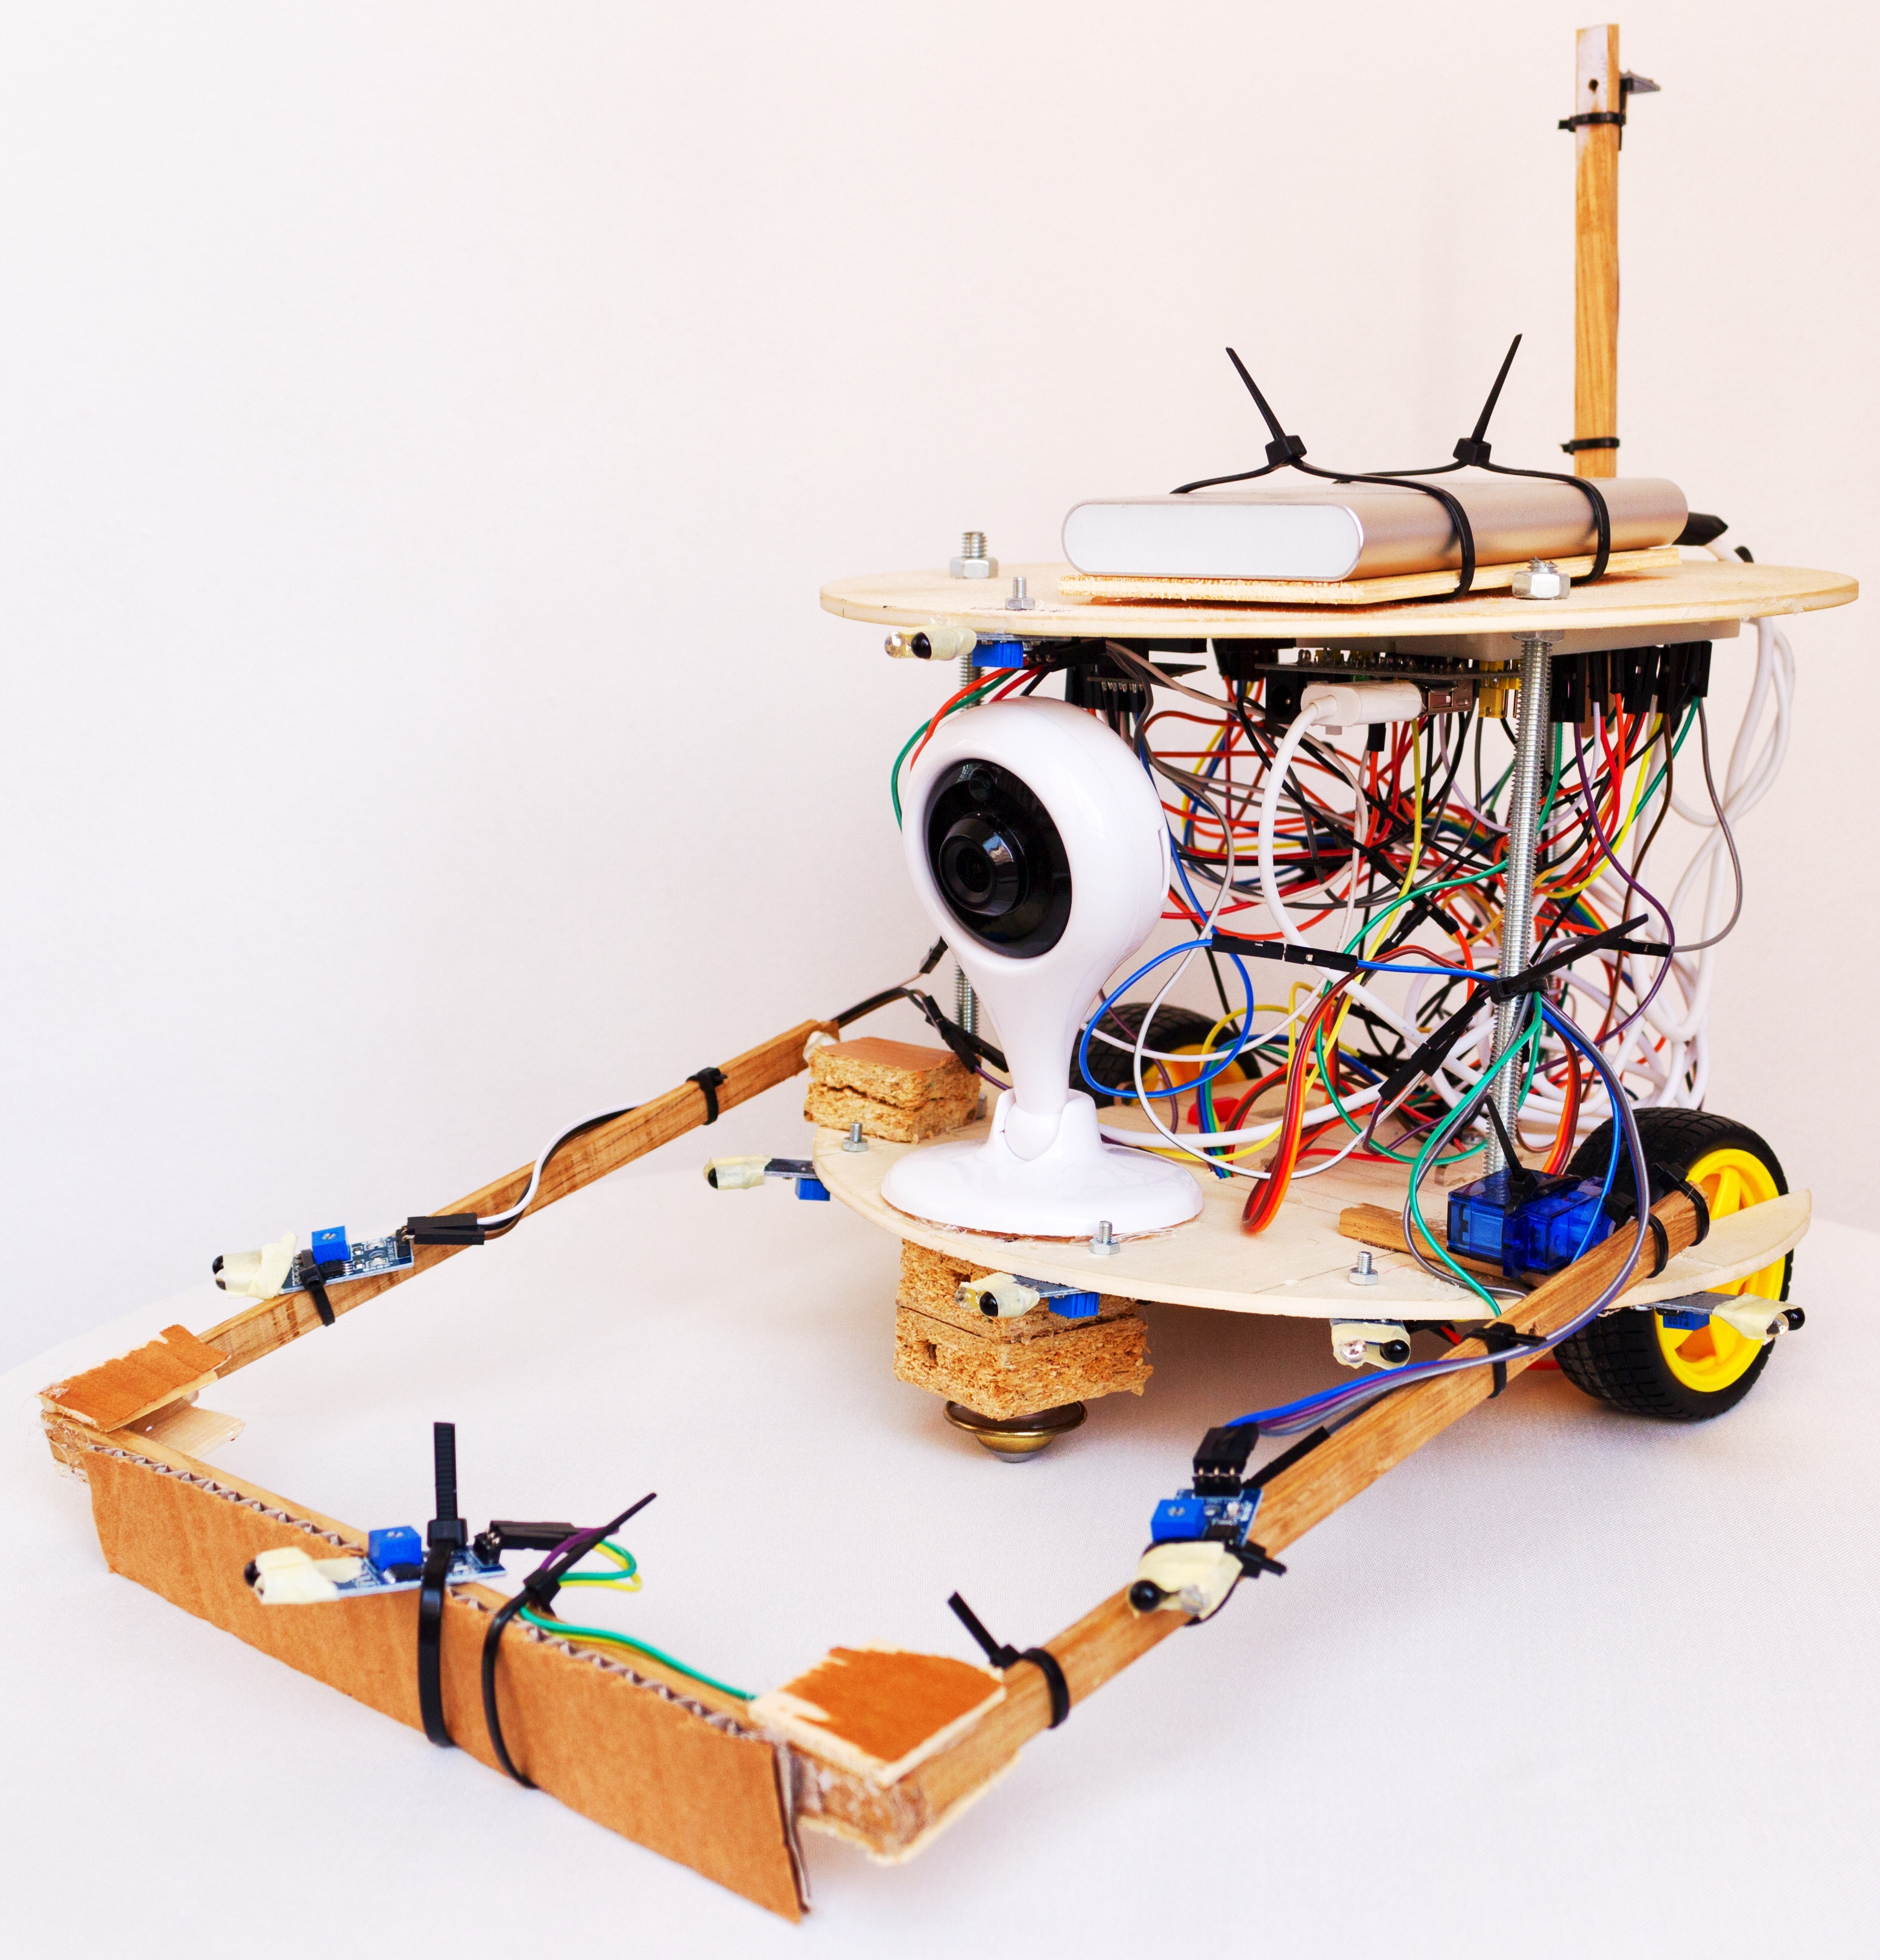
\includegraphics[scale=0.07]{robohenree_1}
\caption{Robohenree}
\label{Fig: robohenree}
\end{center}
\end{figure}

\begin{figure}[H]
\begin{center}
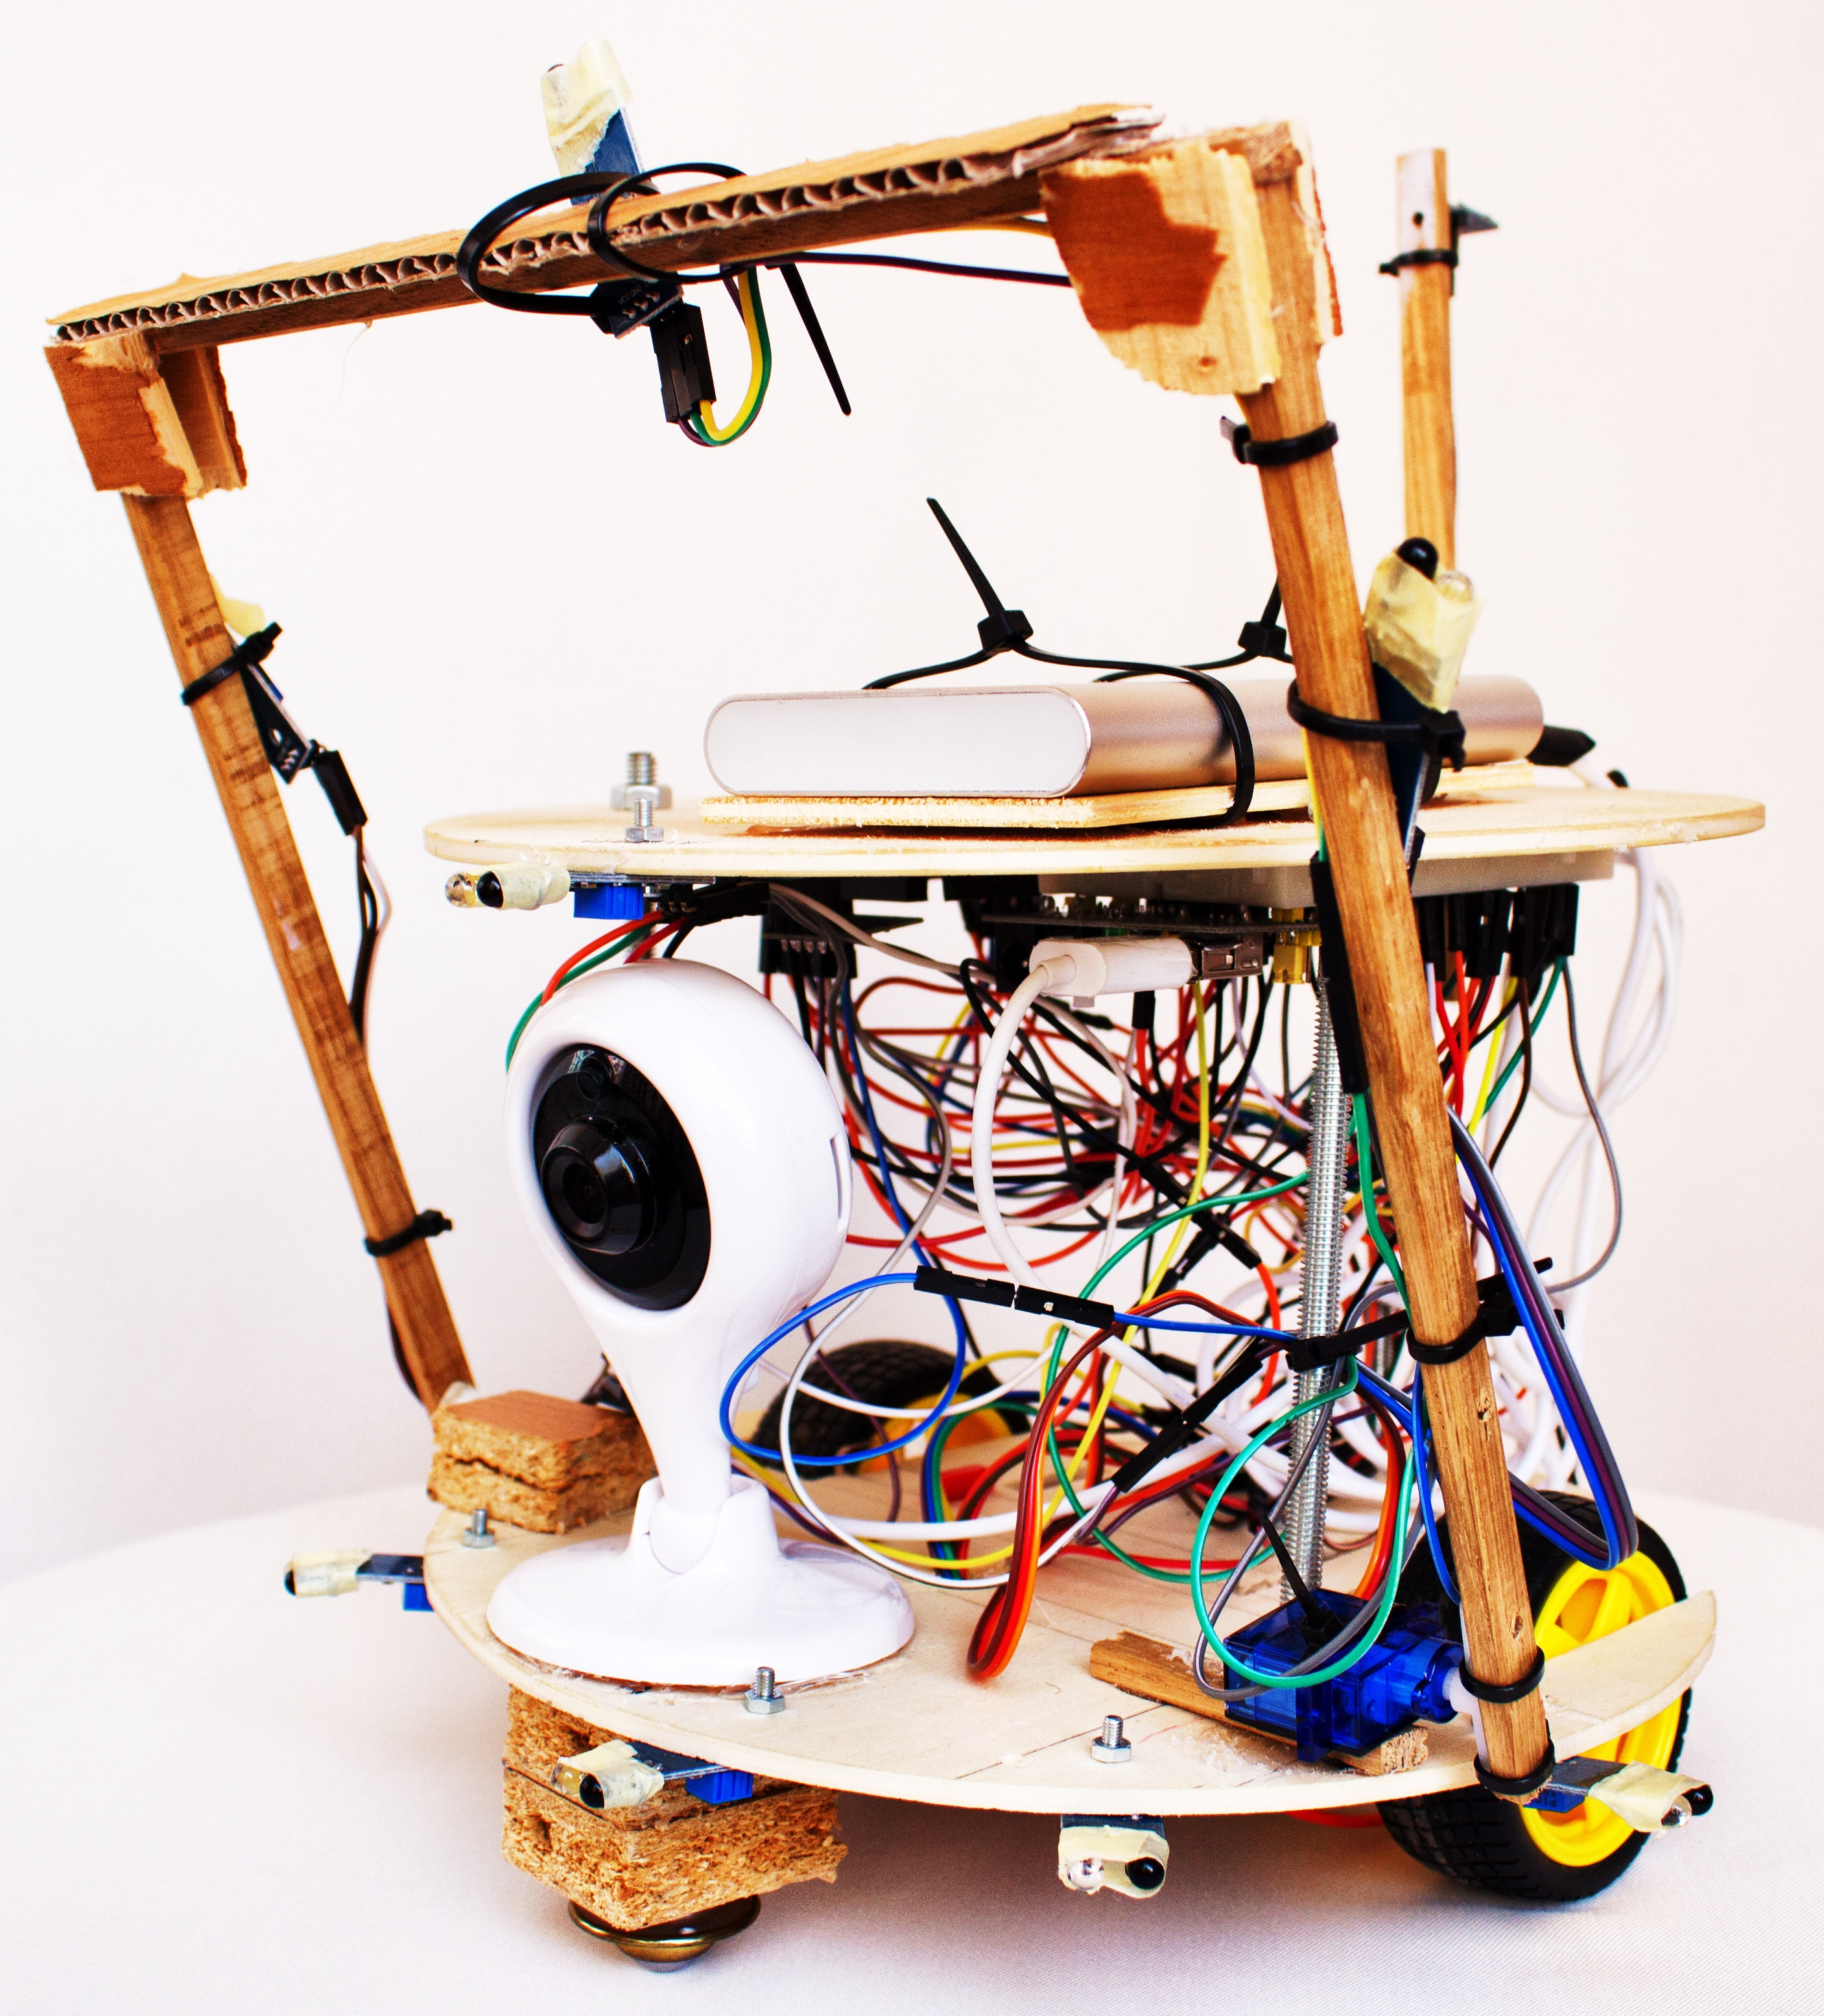
\includegraphics[scale=0.07]{robohenree_2}
\caption{Robohenree in versione aggressiva}
\label{Fig: robohenree}
\end{center}
\end{figure}

\section{Progettazione}
Introduciamo adesso le scelte progettuali fatte per RoboHenree. Come già accennato in precedenza, la scelta di Arduino ha imposto lo sviluppo di un'architettura client-server in cui Arduino, ovvero il client, comunica costantemente con il server che, secondo una politica ben definita, comunica ad Arduino quali azioni compiere. 

Per quanto riguarda gli approcci usati per la progettazione del robot, si è deciso che, per la competizione proposta, un mix di approcci reattivo e pianificato sarebbe stata la soluzione migliore. Infatti, il robot è in grado, grazie ai sensori ad infrarosso, di poter evitare gli ostacoli in maniera reattiva, ma mantenendo comunque un andamento e degli obiettivi da raggiungere decisi da una fase di pianificazione server-side.

Il sistema che abbiamo sviluppato prevede quindi le seguenti parti.
\begin{itemize}
	\item Arduino: percepisce il mondo circostante, agendo con un approccio reattivo in base alla percezione del mondo. Esso ha comunque delle regole da rispettare che gli vengono dettate del server.
	\item Server: decide quali azioni il robot deve compiere (movimento, rotazioni, presa/rilascio oggetti), secondo un piano definito a priori. 
	\item Camera: viene invocata dal server per acquisire immagini del mondo, farne un'elaborazione in base a dei parametri specificati, e di conseguenza permettere al server di dare un comando specifico al robot.
\end{itemize} 


L'architettura è quindi rappresentabile da uno schema del genere.

\begin{center}
	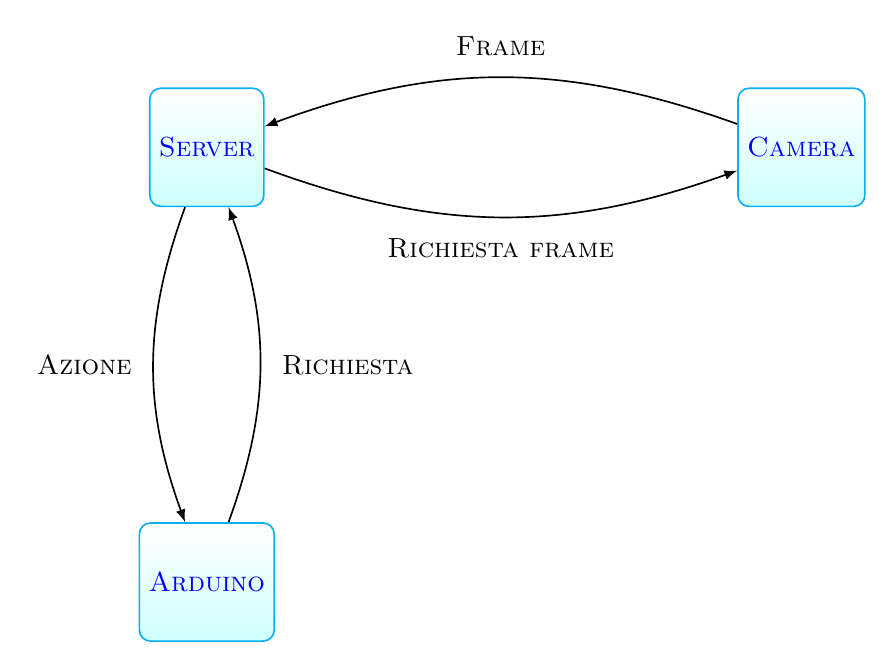
\begin{tikzpicture}[-latex, auto,node distance=4cm and 6cm, semithick,state/.style={rectangle, rounded corners, minimum width=1.7cm, minimum height=1.5cm,  top color=white,bottom color=processblue!20, draw, processblue, text=blue,minimum width=1cm}]
		\node[state] (A) {\textsc{Server}};
		\node[state] (B) [below = of A] {\textsc{Arduino}};
		\node[state] (C) [right = of A] {\textsc{Camera}};
		\path (A) edge [bend right = 20] node[left=0.15cm] {\textsc{Azione}} (B);
		\path (B) edge [bend left = -20] node[right=0.15cm] {\textsc{Richiesta}} (A);
		\path (A) edge [bend right = 20] node[below=0.15cm] {\textsc{Richiesta frame}} (C);
		\path (C) edge [bend left = -20] node[above=0.15cm] {\textsc{Frame}} (A);
	\end{tikzpicture}
\end{center}

Introduciamo adesso le varie parti della progettazione di RoboHenree: diagrammi UML, macchina a stati finiti, e schema circuitale.

\subsection{UML}
UML, acronimo di Unified Modeling Language, è un linguaggio di modellizzazione utilizzato in ingegneria del software per documentare soluzioni progettuali di sistemi anche complessi. L’UML è, dunque, un metodo per descrivere l’architettura di un sistema in dettaglio. La sua vera forza consiste nel fatto che il processo di disegno del sistema può essere effettuata in modo tale che i clienti, gli analisti, i programmatori e chiunque altro sia coinvolto nel sistema di sviluppo possa capire ed esaminare in modo efficiente il sistema e prendere parte alla sua costruzione in modo attivo. Inoltre è basato sul paradigma orientato agli oggetti. 

Prima di scrivere il codice per RoboHenree, abbiamo tracciato dei diagrammi UML per sapere quali classi creare, con quali metodi, e capirne la comunicazione. Questo è il primo passo da compiere prima di iniziare la realizzazione di qualsiasi progetto perché rappresenta una linea guida per la stesura del codice ed evitare quindi di scrivere un programma poco leggibile e talvolta errato. 

Gli schemi UML realizzati sono proposti nelle figure.


\subsection{Pianificazione delle azioni}
\label{Sec: FSM}

Una macchina a stati finiti è un modello che permette di descrivere con precisione il comportamento di un sistema. Le caratteristiche di una macchina a stati finiti fanno si che un suo utilizzo permette di avere un controllo totale su un sistema. Nel nostro caso ci permette di sapere in che stato si trova il robot, in qualsiasi condizione.

RoboHenree viene comandato secondo una sequenza di azioni definite dalla macchina a stati finiti mostrata in figura.

\begin{center}
	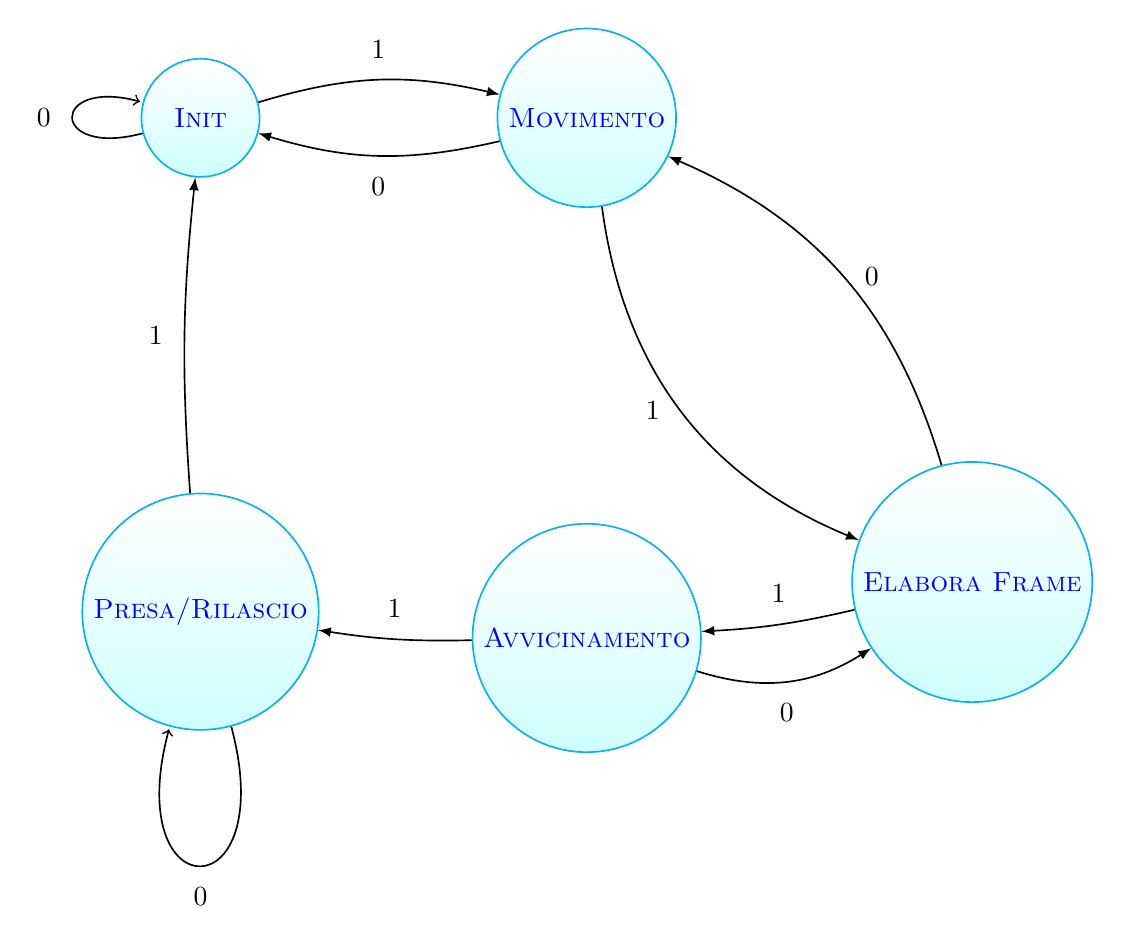
\begin{tikzpicture}[-latex, auto, node distance=4cm and 3cm, semithick, state/.style={circle, top color=white, bottom color=processblue!20, draw, processblue, text=blue, minimum width=1.5cm}]
		\node[state] (A) {\textsc{Init}};
		\node[state] (B) [right = of A] {\textsc{Movimento}};
		\node[state] (C) [below right = of B] {\textsc{Elabora Frame}};
		\node[state] (D) [below = of B] {\textsc{Avvicinamento}};
		\node[state] (E) [below = of A] {\textsc{Presa/Rilascio}};
		\path (A) edge [loop left] node[left=0.15cm] {$0$} (A);
  		\path (A) edge [bend left = 15] node[above=0.15cm] {$1$} (B); 
  		\path (B) edge [bend left = 15] node[below=0.15cm] {$0$} (A);  		
  		\path (B) edge [bend right] node[left=0.15cm] {$1$} (C);
  		\path (C) edge [bend right = 25] node[right=0.15cm] {$0$} (B);
  		\path (C) edge [bend left = 5] node[above=0.15cm] {$1$} (D);
  		\path (D) edge [bend right = 25] node[below=0.15cm] {$0$} (C);
  		\path (D) edge [bend left = 5] node[above=0.15cm] {$1$} (E);
  		\path (E) edge [loop below = 3] node[below=0.15cm] {$0$} (E);
  		\path (E) edge [bend left = 5] node[left=0.15cm] {$1$} (A);
	\end{tikzpicture}
\end{center}


Analizziamo ora i quattro stati della macchina a stati finiti e vediamo a causa di quale evento evolve ogni singolo stato.

\begin{itemize}
	\item \textbf{Init}: questa è la fase in cui il robot dovrà ruotare fino a quando non raggiunge un determinato angolo; se l'angolo indicato non viene raggiunto, allora il robot continuerà a ruotare fino a quando non raggiunge l'angolo.
	\item \textbf{Movimento}: il robot si muove lunga una traiettoria rettilinea, evitando ostacoli in modo reattivo; inoltre nel momento in cui la sua angolazione non è quella indicata in init, allora si re-orienta, tornando allo stato init;
	\item \textbf{Elabora frame}: il server acquisisce un frame del mondo, lo elabora e determina se ha individuato l'area target (qualunque sia l'area, oggetti o goal); se l'elaborazione del frame mi dà esito negativo, allora ritorno in modalità movimento, altrimenti imposto il robot in modalità avvicinamento;
	\item \textbf{Avvicinamento}: il robot diminuisce la velocità dei suoi motori, avvicinandosi all'oggetto o all'area individuata; il sistema ha sempre bisogno di acquisire frame in questa fase, in quanto cerca di allinearsi alla traiettoria verso l'oggetto; se l'oggetto o l'area risultano essere ancora lontani, allora torna allo stato precedente, altrimenti passa allo stato successivo;
	\item \textbf{Presa/Rilascio}: il robot si trova vicino l'oggetto o l'area, inizia muoversi molto lentamente fino a quando non lo percepisce. Se lo percepisce, allora lo prende o lo rilascia, altrimenti continua a muoversi lentamente fino a quando non lo percepisce; nel momento in cui cattura o rilascia l'oggetto allora è pronto per un nuovo percorso da fare, passando allo stato init.
\end{itemize}

\subsection{Schema circuitale}
Lo schema circuitale rappresenta il riassunto di tutte quante le componenti che costituiscono il nostro robot. Per poter realizzare tale schema abbiamo utilizzato il software open source Fritzing che, tramite interfaccia grafica permette di comporre le varie parti elettroniche presenti in un circuito. Di seguito viene mostrato lo schema del nostro progetto, realizzato a partire dall’Arduino Mega 2560 R3 e assemblato a partire dalle componenti descritte alla sezione \ref{subsec: sensori}.

\begin{figure}[H]
	\begin{center}
	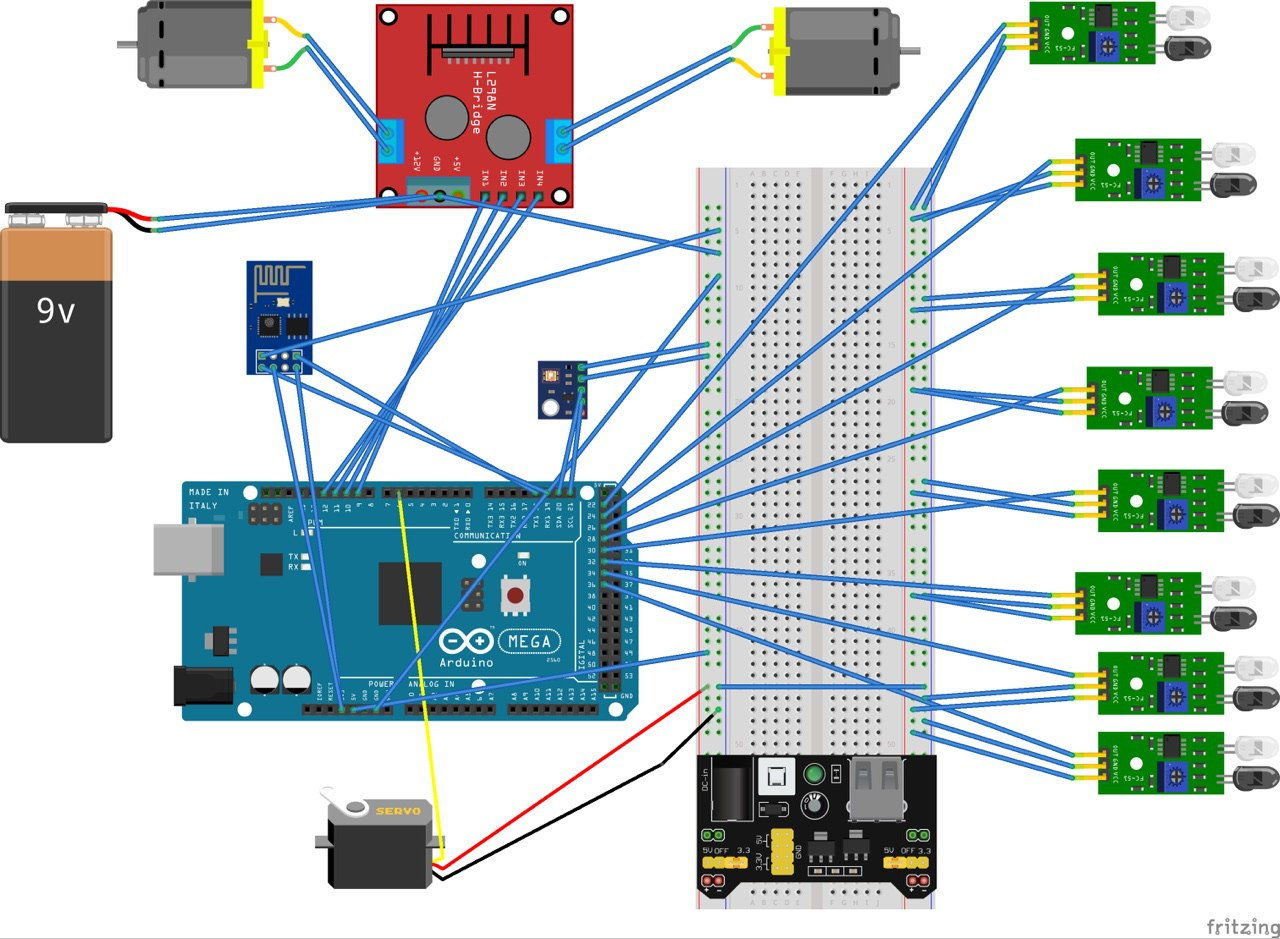
\includegraphics[scale=0.15]{circuito}
	\caption{Schema circuitale di RoboHenree}
	\label{Fig: circuito}
	\end{center}
\end{figure}

\section{Algoritmi e implementazione}

\subsection{Navigazione}
Ci occupiamo adesso di una parte molto importante nello sviluppo del robot: la navigazione all'interno della mappa. Tale parte risulta essere molto importante in quanto, avere un buon algoritmo per la navigazione del robot, può permettere di ridurre il tempo impiegato per raggiungere i vari obiettivi, aumentando così il punteggio per la classifica finale.

Durante lo sviluppo del progetto, gli approcci per la navigazione proposti e testati sono stati due: uno basato sull'algoritmo A* con ciclo percezione-pianificazione-azione, l'altro basato su un approccio reattivo con una guida sui movimenti da fare.

Il secondo approccio ci è sembrato fin da subito il migliore, in quanto il primo richiedeva una precisione negli spostamenti, e un tempo di ciclo di esecuzione elevato. Notiamo inoltre come un'elevata precisione richiede anche l'uso di più sensori, cosa che ci potrebbe fare sforare il budget imposto dalla competizione.

Il mix portato dal secondo approccio ci permette invece di sfruttare la bussola a pieno. Infatti l'idea che sta alla base del nostro algoritmo di movimento è quella di muoversi verso un'area target muovendosi e rispettando sempre un certo valore dato dalla bussola. Infatti a partire da una posizione di partenza nota, si determina l'angolo con il quale il robot punta verso l'altra area in posizione nota. Tale angolo lo abbiamo chiamato \textbf{angolo target}. Dopo aver preso i dati sugli angoli, allora l'algoritmo di navigazione prevede una serie di movimenti in avanti con un'eventuale re-orientazione durante il percorso. La re-orientazione viene dettata dal server, che terrà conto di quando effettuarla.

Questo approccio inoltre permette di avere un robot totalmente reattivo per quanto riguarda gli ostacoli da evitare, con l'unico sforzo di definire una politica ben precisa a priori. 

Risulta quindi chiaro che un aspetto positivo di questo approccio è il non dover per forza tarare gli attuatori ad un grado di precisione elevato, in quanto una fase di re-orientazione ci permette di ritornare lungo la strada verso l'area target. Il problema di questo approccio si presenta nel momento in cui campi magnetici esterni influenzano la bussola, facendo rilevare dati sbagliati, con la possibilità che un'eventuale re-orienting non vada a buon fine.

Figure che spiegano il concetto dell'algoritmo di movimento sono le Figure \ref{Fig: movimento_1}, \ref{Fig: movimento_2}, \ref{Fig: movimento_3}, \ref{Fig: movimento_4}.

\begin{figure}[H]
	\begin{center}
	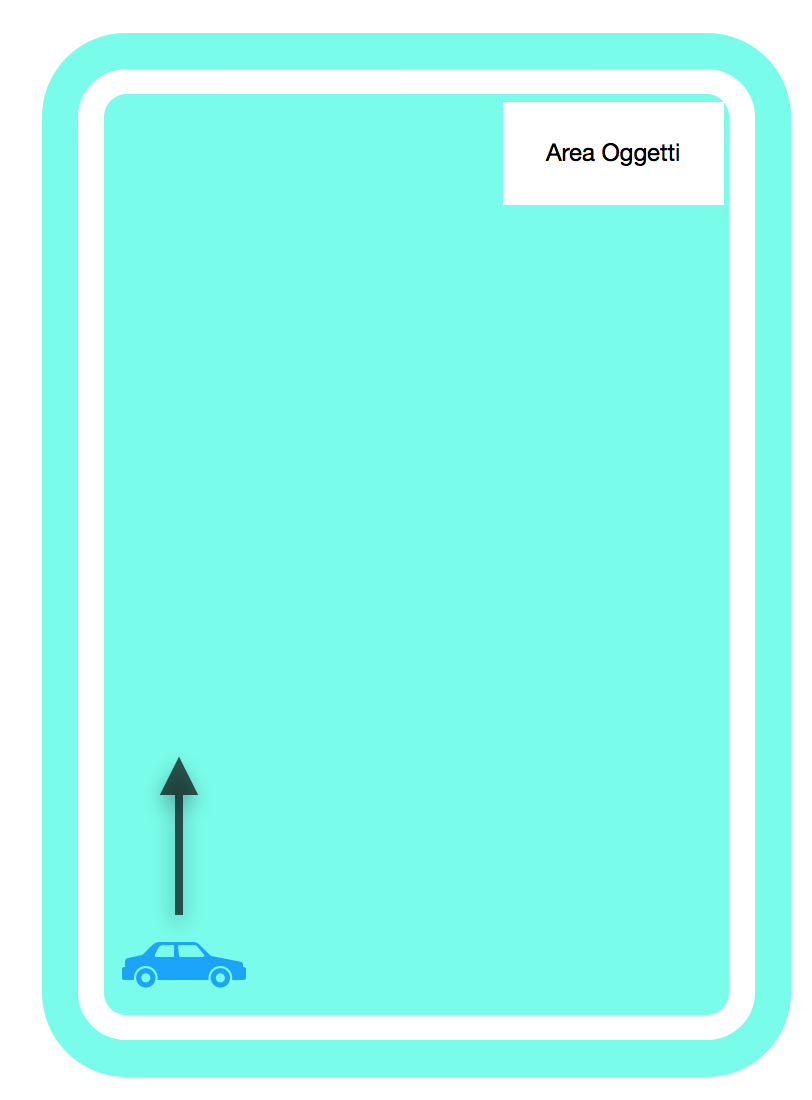
\includegraphics[scale=0.3]{movimento_1}
	\caption{RoboHenree in posizione iniziale}
	\label{Fig: movimento_1}
	\end{center}
\end{figure}


\begin{figure}[H]
	\begin{center}
	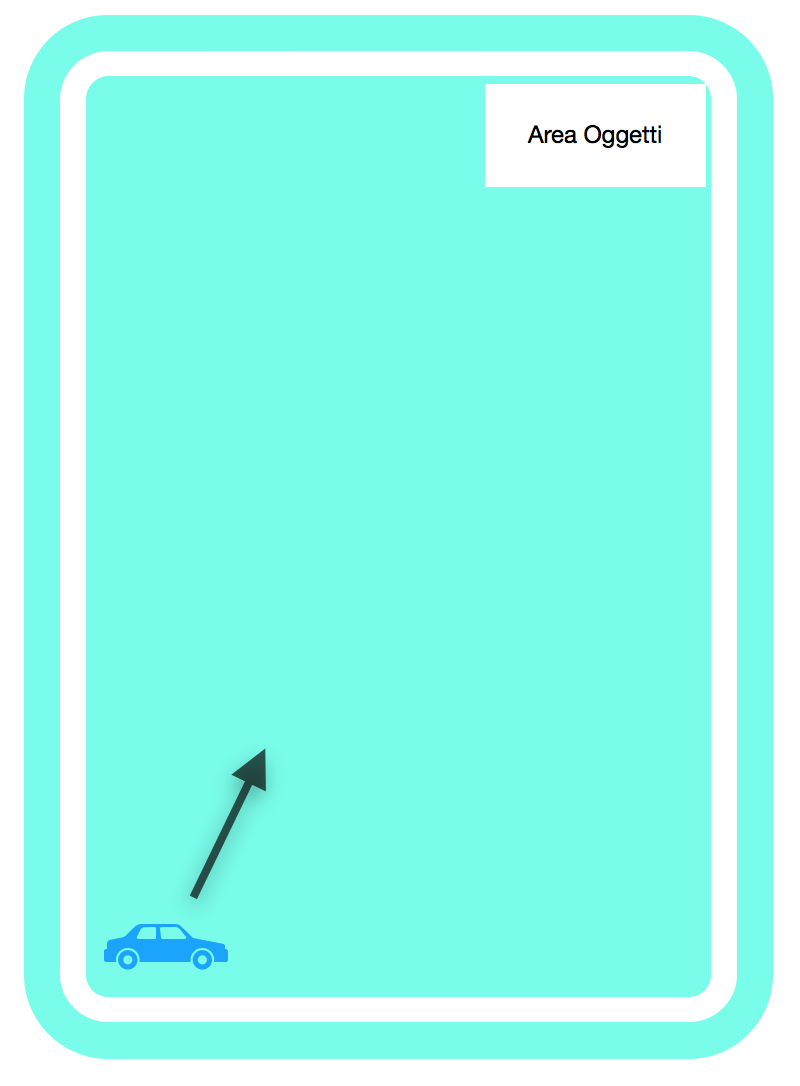
\includegraphics[scale=0.3]{movimento_2.png}
	\caption{RoboHenree orientato verso l'area oggetti}
	\label{Fig: movimento_2}
	\end{center}
\end{figure}


\begin{figure}[H]
	\begin{center}
	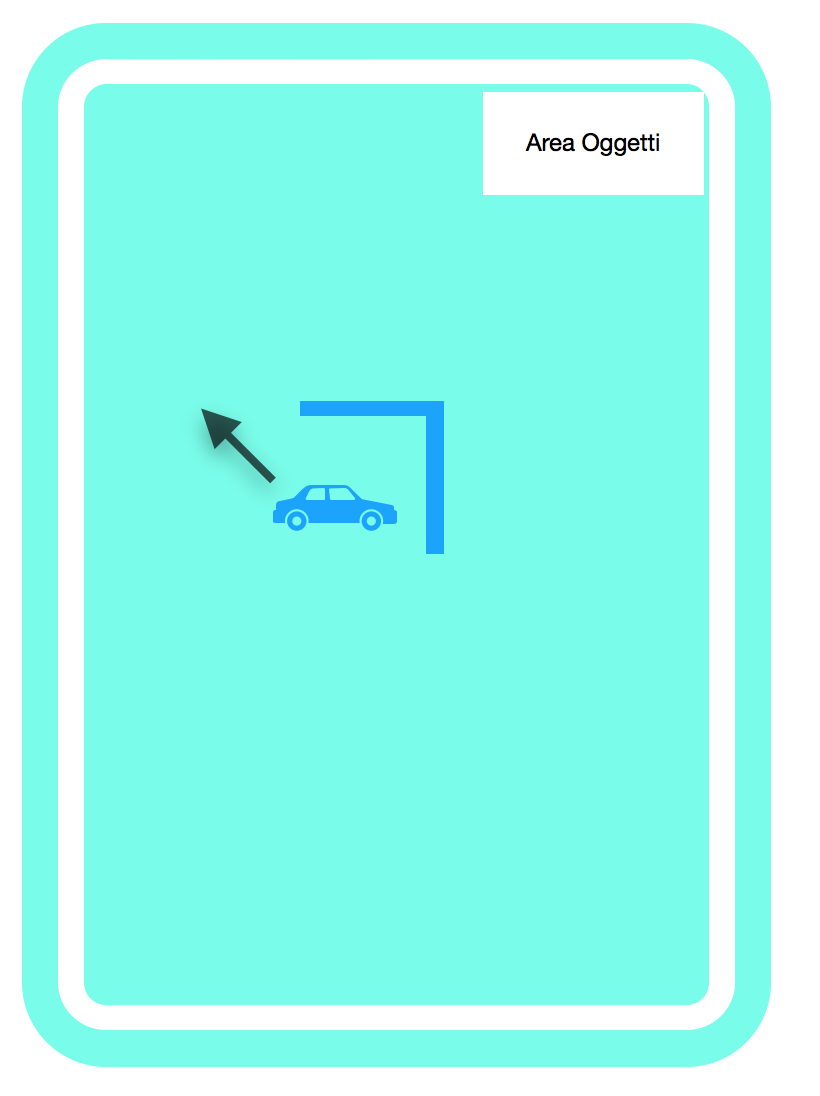
\includegraphics[scale=0.3]{movimento_3.png}
	\caption{RoboHenree che evita gli ostacoli reattivamente}
	\label{Fig: movimento_3}
	\end{center}
\end{figure}

\begin{figure}[H]
	\begin{center}
	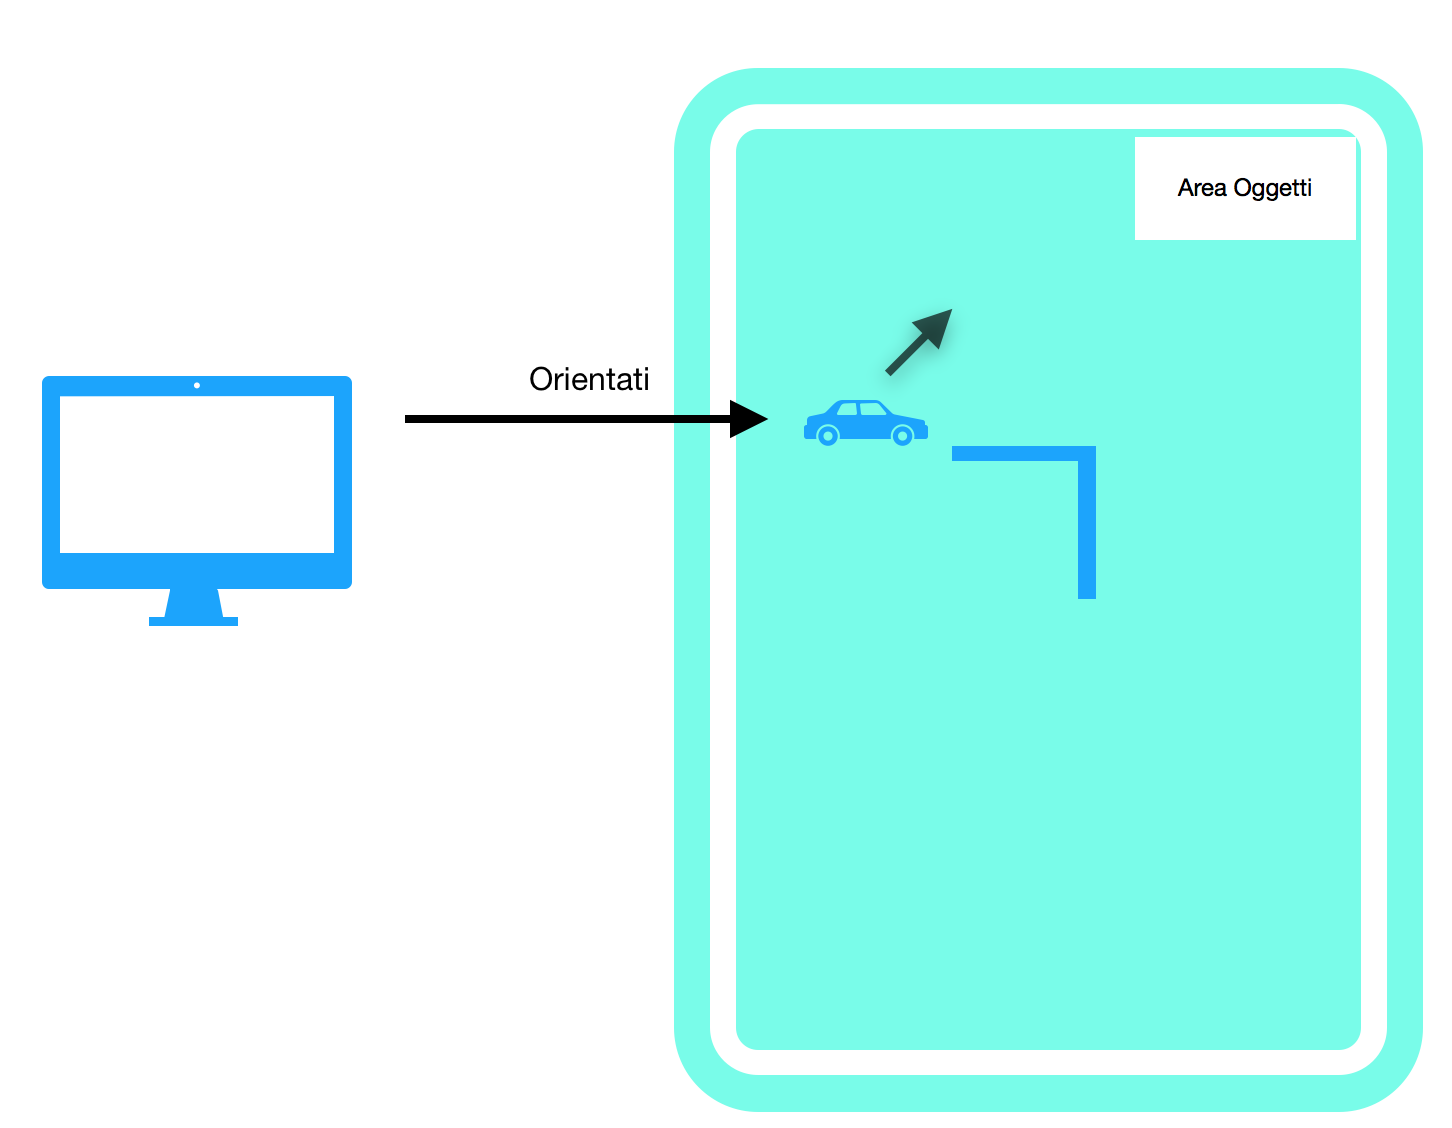
\includegraphics[scale=0.3]{movimento_4.png}
	\caption{RoboHenree che si re-orienta secondo il comando del server}
	\label{Fig: movimento_4}
	\end{center}
\end{figure}

\subsection{Comunicazione con il server}

L'architettura scelta per il robot prevede necessariamente la comunicazione tra un client, Arduino, ed un server che comunicano con una connessione TCP. In particolare:
\begin{itemize}
	\item Arduino avvia una nuova connessione TCP, mandando una richiesta al server su una determinata porta.
	\item Il server in ascolto su una porta e accetta di stabilire una connessione, processando la richiesta del client ed eventualmente rispondere.
\end{itemize}

La comunicazione fra Arduino e il server è permessa dal modulo Wi-Fi ESP8266 presentato nella sezione \ref{subsec: sensori}. Il modulo prevede dei comandi di default che gli consentono di instaurare una connessione TCP con un server. 

Lato server è stata implementata una classe, \textbf{Robot}, che permettesse di aprire la connessione tra Arduino e il server. Il server ascolta eventuali richieste di connessione sulla porta 1931.

Client e server si scambiano costantemente informazioni del tipo:
\begin{itemize}
	\item \textbf{Sensoriali}: il client comunica al server lo stato del mondo secondo i suoi sensori.
	\item \textbf{Comandi}: il server comunica al client quali azioni compiere nel mondo.
\end{itemize}

I messaggi che client e server si scambiano sono in formato \textbf{JSON}, un formato di testo completamente indipendente dal linguaggio di programmazione, ma che utilizza convenzioni conosciute dai programmatori di linguaggi della famiglia del C, come Python per l'appunto.



































\end{document}